\pagestyle{fancy}
\fancyhead[LE,LO]{OCR A Level - Computer Science NEA}
\fancyhead[RE,RO]{Jonathan Kasongo}

\chapter{Analysis of the problem}

\section{Problem Identification}
The game of chess has skyrocketed in terms of popularity
recently, so much so that half of my school now spend their
break times playing each other on \url{chess.com}. Chess 
is a strategy board game with the end goal being to checkmate
the opponent's king. \cite{rules} This means that capture of 
the opponent's king is inevitable upon the next move. The 
game also involves \textbf{no} elements of luck and the 
outcome of the game is soley dependent on the actions of the
player. Moreover, the game of chess is known to be very
hard to master with many of the best chess
\textit{Grandmasters} starting training from the
ages of 7-8 \cite{Magnus}. The game of chess has an average
of 35 moves \cite{branch} per position. This means that 
if one wants to think three moves ahead of his opponent
he must consider $42,875$ positions in total! This is
simply not possible for a human, however for a computer
this task is something that could be done in less than
1 second. By leveraging the high computational power
of modern computers, I aim to write a chess engine that
is able to beat an average human chess player 9 times
out of 10.\\

Whilst chess prodigies and Grandmasters dedicate their entire
lifes to improving their chess abilities, using high order 
thinking processes, experience and strategical tactics to play
the best move in a position we may simply use a brute-force 
style of play, in which we consider all legal moves from a 
given position and simply choose the one that gives the most
advantageous position even if our opponent doesn't make any 
mistakes.

% https://en.wikipedia.org/wiki/World_Chess_Championship_1984%E2%80%931985
% https://www.chessprogramming.org/Branching_Factor
\section{Stakeholders}
% https://www.nytimes.com/2022/06/17/crosswords/chess/chess-is-booming.html
One of the students at my school who plays chess regularly is 
John Arco. John Arco is a 17 year old male with a passion for chess.
John has a rating of roughly 1000 ELO but wishes 
to improve to a higher rating and beat all of his 
classmates. John is also very competitive and wishes to 
\textbf{guarentee} that none of his classmates can beat him.
The use of a strong chess engine is one method to ensure
that John Arco always beats his classmates and requires little
to no effort on his part, all he has to do is replicate the 
moves played by his opponent on the engine's board and he 
will simply replicate the computer's moves. 
\footnote{I do realise that this is considered cheating,
however we intend to use this engine completely offline
in unrated friendly games against close friends. 
I do not advocate cheating in any way shape or form.}
Moreover using a chess engine can also be highly educational as
we may learn new ideas or moves from the engine that we may have
never considered previously. Even Magnus Carlsen
has openly said that he has learnt new ideas from chess engines.
\cite{lex} This means the engine is to serve 2 purposes,
the first is ensure that John Arco remains undefeated 
against his classmates, and the second is to improve John Arco's
chess ability by exposing him to new and unique tactics that 
he wouldn't have thought of otherwise. The construction of 
a strong chess engine will be able to solve both problems
effectively, providing both educational benefits and 
competitive benefits also.

\section{Research the problem}
To begin research it is first nescessary to get a higher level understanding
of how a chess engine works. To learn about this topic
I made use of resources like \url{https://www.chessprogramming.org/Main_Page}
and \url{https://www.talkchess.com/forum/index.php}, citations will be 
given accordingly. The following subsections will act to be 
a brief summary of the research I conducted on understanding
how to write a chess engine.\\

Any chess engine must be comprised of these 3 fundamental components:
\begin{itemize}
  \item \textit{Legal move generation}
  \item \textit{Evaluation functions}
  \item \textit{Searching algorithms}
\end{itemize}

We will explore each of these components in detail, however 
if you have never come across the term "bitboards" in 
relation to chess programming, I strongly 
encourage you to read the next subsection.

\subsection*{Bitboards}
To understand the following algorithms it is nescessary to 
have an adequate understanding on \textbf{\textit{bitboards}}.
If you already understand this concept please skip this 
subsection entirely, otherwise I will provide a brief 
introduction to the idea here. Some helpful resources can be
found here \cite{bitboards}.\\

Bitboards are a way to represent the state of the 
chess board with a 64 bit number. Consider the following 
chess position.

\begin{figure}[h]
  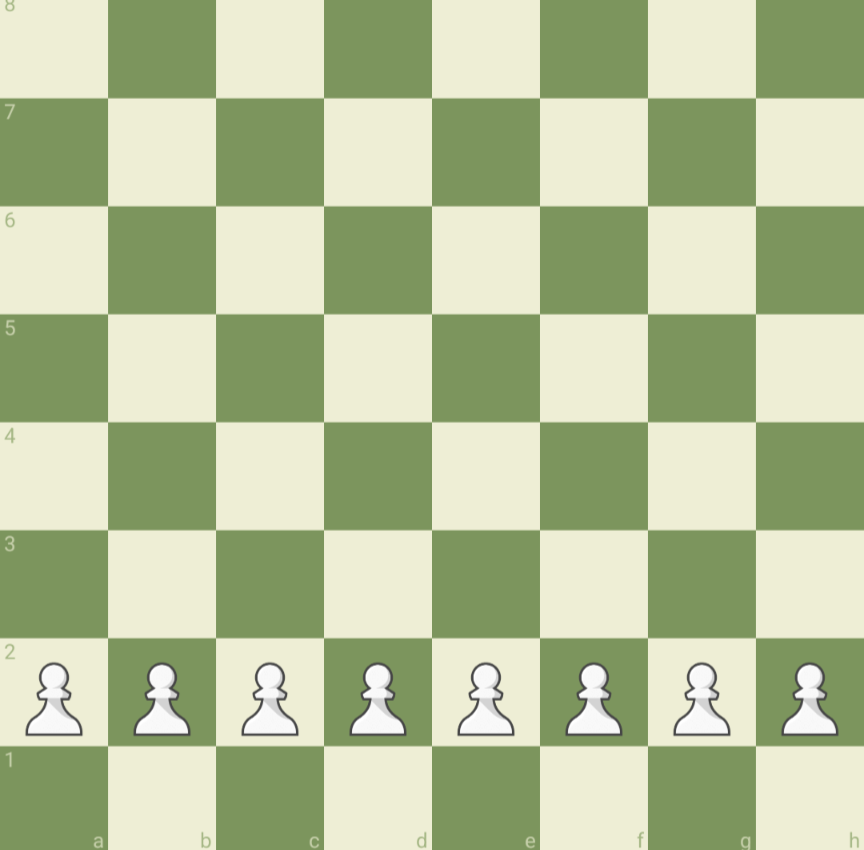
\includegraphics[scale=0.25]{White_Pawns_start.png}
  \centering
  \caption{Starting position for white pawns}
  \label{whitepawns}
\end{figure}

Notice that a chess board has dimensions
$(8 \, \textrm{x} \, 8)$ and 64 squares. Furthermore, 
each of the squares in figure \ref{whitepawns} exists 
in one of two states: There either is a white pawn on
this square or there is not. This innate similarity to 
the binary numbering system motivates one to consider the 
use of binary to represent a chess board. We can take a 
64 bit unsigned integer and have each \texttt{0} 
represent the lack of a piece and similarly 
have each \texttt{1} represent the existance of a piece on 
this square.\\

Consider the following code snippet.\footnote{The importing
of the numpy library has been omitted for clarity.}\\

\begin{minted}[linenos, bgcolor=lightgray]{Python}
  # For the rest of this paper i64 will refer to the 
  # unsigned 64 bit integer
  i64 = np.uint64
  WhitePawn = i64(0b        # Dots represent 0,
                  00000000  # . . . . . . . .
                  00000000  # . . . . . . . .
                  00000000  # . . . . . . . .
                  00000000  # . . . . . . . .
                  00000000  # . . . . . . . .
                  00000000  # . . . . . . . .
                  11111111  # 1 1 1 1 1 1 1 1
                  00000000) # . . . . . . . .
\end{minted}

Each bit in the \texttt{WhitePawn} variable represents the
state of a square like we saw previously, this allows us to 
store the state of the board with 12, 64 bit numbers 
(6 piece types in chess, and 2 players). Modern computers
typically have register sizes of 64 bits or greater, 
meaning that we may easily and quickly manipulate these 
bitboards in order to generate legal moves for a position.
We will consider how we may leverage bitboards for legal 
move generation in the following subsection.

\subsection*{Legal move generation}
Legal move generation is the first step to writing a strong
chess engine, in this component we wish to 
find a way to feed in a position to a computer program and have it 
output to us all of the possible legal moves available in this position.
The study of move generation algorithms in the chess programming world 
is still very nascant, with one of the newest algorithms
being discovered in 2017 \cite{bm}. The two algorithms I
decided to spend time researching were
\textit{Hyperbola quintessence} and 
\textit{Magic bitboards} because they are the standard 
accepted algorithms for the top chess engines 
\cite{stockfish}.\\

Hyperbola quintessence is an algorithm used to generate moves
for sliding pieces \footnote{That is the queen, bishop and rook.}.
It makes use of bit manipulation tricks to generate these moves
in $O(1)$ time.
